%pdflatex --shell-escape -interaction=nonstopmode %.tex

\documentclass[10,pt]{journal}

\usepackage[latin1]{inputenc}
\usepackage{tikz}

\usepackage[miktex]{gnuplottex}
\usepackage{mathpazo}

\usepackage{geometry}

\geometry{top=2.5cm,bottom=2.5cm}
% GNUPLOT required
\begin{document}
\pagestyle{empty}

\begin{center}
  {\LARGE Command}\\
  {\small \today}
\end{center}

\begin{figure}[h]
  \begin{center}
    \begin{minipage}{0.6\linewidth}
      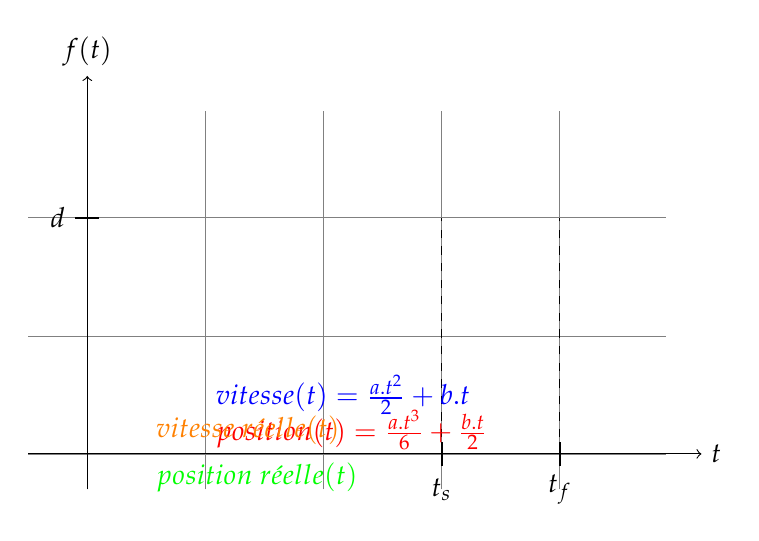
\begin{tikzpicture}[scale=1.5,domain=0:5]
        \draw[very thin,color=gray] (-0.5,-0.3) grid (4.9,2.9);
        \draw[->] (-0.5,0) -- (5.2,0) node[right] {$t$};
        \draw[->] (0,-0.3) -- (0,3.2) node[above] {$f(t)$};
        
        \draw[thick] (3,-0.1) -- (3,0.1);
        \draw[thick] (4,-0.1) -- (4,0.1);
        \draw[dashed] (3,0) -- (3,2) node at (3,-0.3) {$t_s$};
        \draw[dashed] (4,0) -- (4,2) node at (4,-0.3) {$t_f$};
        
        \draw[thick] (0.1,2) -- (-0.1,2) node[left] {$d$};
        
        \draw[color=blue,thick] plot[id=x,domain=0:3] function{-0.444444*x*x+1.333333*x}
        node[right] at +(1,0.5) {$vitesse(t) = \frac{a.t^{2}}{2} + b.t$};
        \draw[color=blue,thick] plot[id=x,domain=3:4] function{0};
        
        \draw[color=red,thick] plot[id=x,domain=0:3] function{-0.148148*x*x*x+0.666666*x*x}
        node[right] at +(1,0.2) {$position(t) = \frac{a.t^{3}}{6} + \frac{b.t}{2}$};
        \draw[color=red,thick] plot[id=x,domain=3:4] function{2}; 
        
        \draw[color=green] plot[id=x,domain=0:3.5] function{-0.0932944*x*x*x+0.489795*x*x}
        node[right] at +(0.5,-0.2) {$position~r\acute{e}elle(t)$};
        \draw[color=green] plot[id=x,domain=3.5:4] function{2}; 
        
        \draw[color=orange] plot[id=x,domain=0:3.5] function{-0.279883*x*x+0.979591*x}
        node[right] at +(0.5,0.2) {$vitesse~r\acute{e}elle(t)$};
        \draw[color=orange] plot[id=x,domain=3.5:4] function{0}; 

      \end{tikzpicture}


      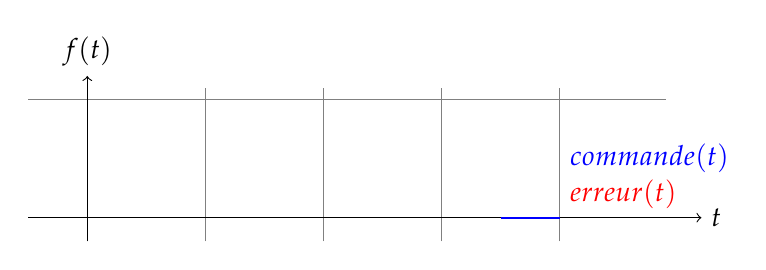
\begin{tikzpicture}[scale=1.5,domain=0:5]
        \draw[very thin,color=gray] (-0.5,-0.2) grid (4.9,1.1);
        \draw[->] (-0.5,0) -- (5.2,0) node[right] {$t$};
        \draw[->] (0,-0.2) -- (0,1.2) node[above] {$f(t)$};
        
        \draw[color=red,thick] plot[id=x,domain=0:3] function{-0.148*x*x*x+0.666*x*x - (-0.0932944*x*x*x+0.489795*x*x) }
        node[right] at (4,0.2) {$erreur(t)$};
        \draw[color=red,thick] plot[id=x,domain=3:3.5] function{2 - (-0.0932944*x*x*x+0.489795*x*x)};
        \draw[color=red,thick] (3.5,0) -- (4,0);  
        
        \draw[color=blue,thick] plot[id=x,domain=0:3] function{2.5*(-0.148*x*x*x+0.666*x*x - (-0.0932944*x*x*x+0.489795*x*x)) }
        node[right] at (4,0.5) {$commande(t)$};
        \draw[color=blue,thick] plot[id=x,domain=3:3.5] function{2.5*(2 - (-0.0932944*x*x*x+0.489795*x*x))};
        \draw[color=blue,thick] (3.5,0) -- (4,0);  
      \end{tikzpicture}
    \end{minipage}
    %\caption{Example of command for $d=2$, $t_f=4$ and $K=2.5$.}
  \end{center}
\end{figure}

\begin{figure}[h]
  \begin{center}
    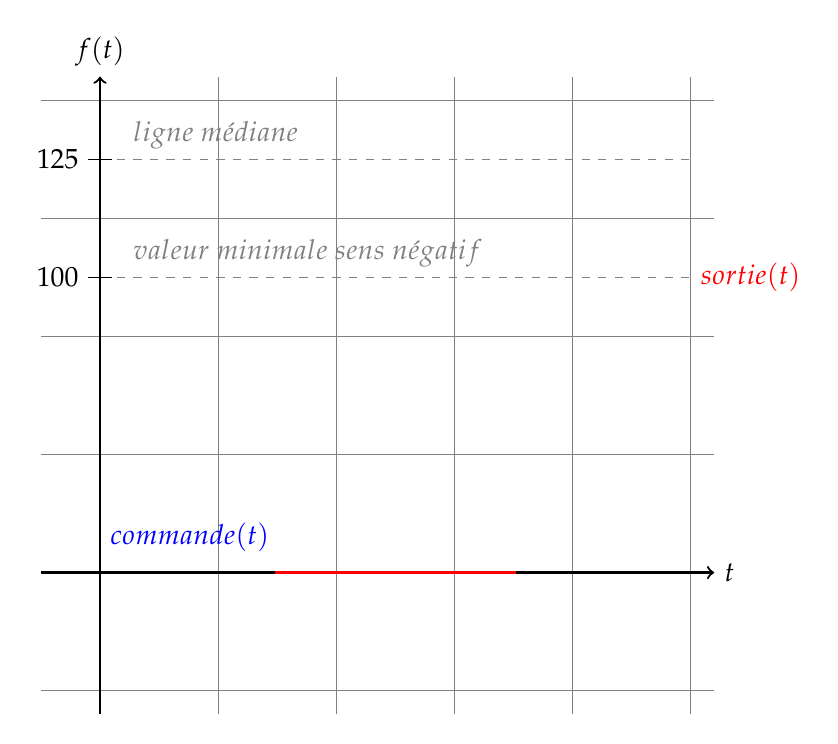
\begin{tikzpicture}[scale=1.5,domain=0:5]
      \draw[very thin,color=gray] (-0.5,-1.2) grid (5.2,4.2);
      \draw[->,thick] (-0.5,0) -- (5.2,0) node[right] {$t$};
      \draw[->,thick] (0,-1.2) -- (0,4.2) node[above] {$f(t)$};
      
      \draw[color=blue,thick] plot[id=x,domain=0:5] function{-0.96*x*x/2 + 2.4*x}
      node[right] at +(0,0.3) {$commande(t)$};
      \draw[color=red,dashed] plot[id=x,domain=0:5] function{-(-0.96*x*x/2 + 2.4*x) +2.5};

      \draw[color=red,thick] plot[id=x,domain=0:1.479379273840342] function{-(-0.96*x*x/2 + 2.4*x) +2.5};
      \draw[color=red,thick] (1.479379273840342,0) -- (3.520620726159658,0);
      \draw[color=red,thick] plot[id=x,domain=3.520620726159658:5] function{-(-0.96*x*x/2 + 2.4*x) +2.5} node[right] at (5,2.5) {$sortie(t)$};
      
      \draw[color=gray,dashed] (0,3.5) -- (5,3.5) node[right] at (0.2,3.7) {$ligne~m\acute{e}diane$};
      \draw[color=gray,dashed] (0,2.5) -- (5,2.5) node[right] at (0.2,2.7)
       {$valeur~minimale~sens~n\acute{e}gatif$};
       
      \draw (0.1,3.5)--(-0.1,3.5) node[left]  {$125$};
      \draw (0.1,2.5)--(-0.1,2.5) node[left]  {$100$};
    \end{tikzpicture}
    %\caption{Example of output, the scale is not respected here.}
  \end{center}
\end{figure}

\end{document}